\documentclass{article}

\usepackage[a4paper,pdftex]{geometry}										% A4paper margins
\setlength{\oddsidemargin}{5mm}												% Remove 'twosided' indentation
\setlength{\evensidemargin}{5mm}

\usepackage[english]{babel}
\usepackage[protrusion=true,expansion=true]{microtype}	
\usepackage{amsmath,amsfonts,amsthm,amssymb}
\usepackage{graphicx}
\usepackage{color}
\usepackage{multirow}
\usepackage{rotating}
\usepackage{caption}
\usepackage{subcaption}
\usepackage{verbatimbox}
%\usepackage[parfill]{parskip}

% ------------------------------------------------------------------------------
% Definitions (do not change this)
% ------------------------------------------------------------------------------
\newcommand{\HRule}[1]{\rule{\linewidth}{#1}} 	% Horizontal rule

\makeatletter							% Title
\def\printtitle{%						
    {\centering \@title\par}}
\makeatother									

\makeatletter							% Author
\def\printauthor{%					
    {\centering \large \@author}}				
\makeatother							

% ------------------------------------------------------------------------------
% Metadata (Change this)
% ------------------------------------------------------------------------------
\title{	\textbf{Computer Networks Practicum}
		}

\author{
		Dimo Stoyanov \& Plamen Dimitrov\\
		dsv200 \& pdv200 \\
		Vrije Universiteit Amsterdam\\	
  %      \texttt{your@email.com} \\
}


\begin{document}
% ------------------------------------------------------------------------------
% Maketitle
% ------------------------------------------------------------------------------
\maketitle

\section{Building a TCP stack}
Our TCP implementation follows strictly the RFC0793 except for the differences explicitly
mentioned in the course requirements.

% Our implementation does not support multiplexing, therefore we made the Socket class singleton

\subsection{TCP Packet}
The TCPPacket class (See~\ref{fig:tcppacket}) was used to wrap a TCP packet. As can be seen
on Figure~\ref{fig:header}, the class implementation matches exactly the header. The class
also has a method for extracting the relevant information from the payload of an IP Packet.

\begin{figure}[h!]
\centering
\begin{subfigure}[b]{0.4\textwidth}
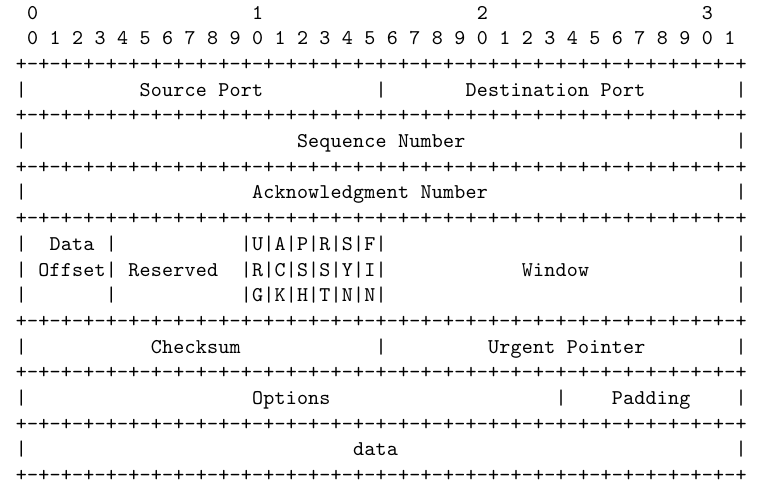
\includegraphics[width=\textwidth]{images/tcp_header}
\caption{TCP header}
\end{subfigure}
\qquad
\begin{subfigure}[b]{0.2\textwidth}
 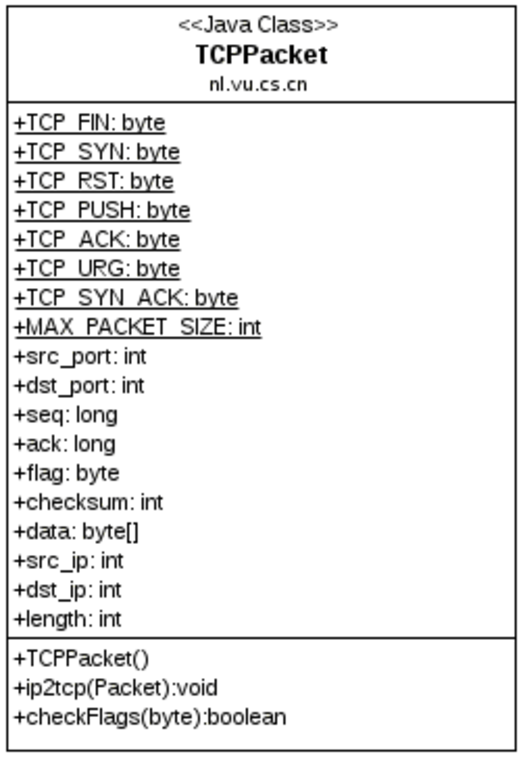
\includegraphics[width=\textwidth]{images/cn_uml}
 \caption{TCPPacket class}
 \label{fig:tcppacket}
\end{subfigure}
\caption{The TCP header and the class used to implement it.}
\label{fig:header}
\end{figure}
\noindent
The types of the TCPPacket's attributes were chosen to adequately represent their ranges and compensate
for the lack of the appropriate unsigned types in Java.
  
\subsection{TCPControlBlock class}
The TCPControlBlock (see Figure~\ref{fig:tcb}) is used to maintain all the information which is needed
for the Socket functioning. The state of the socket is stored in the control block. Figure~\ref{fig:tcb}
shows all the states in our implementation; we will not discuss them in details since they are used
exactly in the way RFC0793 defines them. A socket is uniquely defined based on the control block information.


\begin{figure}[h!]
\centering
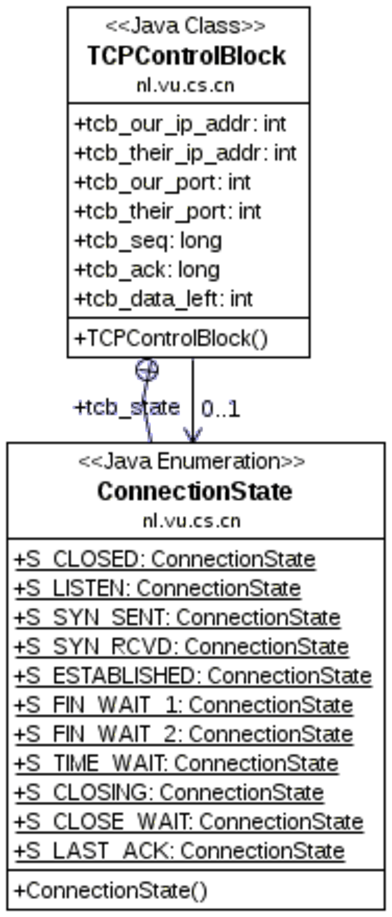
\includegraphics[width=0.2\textwidth]{images/control_block}
\caption{TCPControlBlock class}
\label{fig:tcb}
\end{figure}
  
\subsection{Socket class}
The actual heavy lifting is done in the Socket(see Figure~\ref{fig:socket}) class. As suggested in the assignment, two methods 
(e.g. \textit{send\_tcp\_packet()} and \textit{recv\_tcp\_packet()}) added to the original ones. They carry out the communication
between a socket and the underlying IP layer. The \textit{send\_tcp\_packet()} encodes a TCPPacket into a byte array,
sets the required flags (i.e. sets the PSH flag to on all packets), computes checksums, and transmits the
packet. That method can perform both blocking and non-blocking send. Its non-blocking version is latter 
used for time out detection. The \textit{recv\_tcp\_packet()} method does exactly the opposite to the \textit{send\_tcp\_packet()}:
it receives a packet from the IP layer, checks if the checksum is correct and passes it to the socket
as an instance of the TCPPacket class.


\begin{figure}[h!]
 \centering
 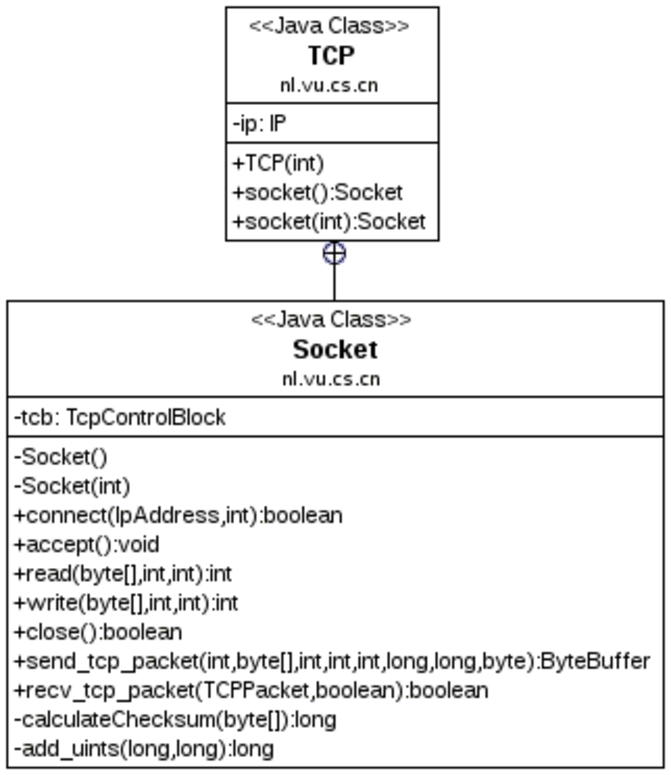
\includegraphics[width=0.5\textwidth]{images/tcp_socket}
 \caption{The TCP and Socket classes}
  \label{fig:socket}
\end{figure}

Another helper method implemented in the Socket class is the \textit{add\_uints()}, used for addition of unsigned 32-bit
integers. These integers are represented as longs (64-bit in Java) and the method prevents the addition/subtraction to
cause overflow or underflow of the 32-bit unsigned integer range.

The main methods in the Socket class are \textit{connect(), accept(), read(), write(), close()}. They have one main feature
in common - the way they deal with errors. To accomplish that, we implemented the state machine from RFC0793. All the methods
require acknowledgement by the other side of every octet they send. In our implementation acknowledgements are sent only in
packets that do not contain any data.


% Our implementation does not support acknowledgement packets
% carrying data.

The \textit{connect()} method, as required, is non-blocking and connects a client socket to a server on given \textit{host}
and \textit{port}.



\section{The Chat Application}
A minimalistic chat application was developed on top of the TCP stack described in the previous chapter.
It consists of a single window used by both a "client" and a "server". The "server" waits for a connection
(e.g. accepts) and the "client" connects to the "server". Because of the lack of multiplexing capabilities
of the TCP implementation, the "server" and the "client" maintain two TCP stacks each. They use one stack
for writing data and one for reading data. The reading is constantly done in separate threads and updates
the GUI upon data arrival.




\end{document}